%----------------------------------------------------------------------------------------
%
% LaTeX-template for degree projects at LNU, Department of Computer Science
% Last updated by Johan Hagelbäck, Mar 2017
% Linnaeus University
%
% License: Creative Commons BY
%
%----------------------------------------------------------------------------------------

%----------------------------------------------------------------------------------------
%	Settings and configuration
%----------------------------------------------------------------------------------------

\documentclass[a4paper,12pt]{article}

\usepackage[T1]{fontenc}
\usepackage{times}
\usepackage[english]{babel}
\usepackage[utf8]{inputenc}
\usepackage{dtklogos}
\usepackage{wallpaper}
\usepackage[absolute]{textpos}
\usepackage[top=2cm, bottom=2.5cm, left=3cm, right=3cm]{geometry}
\usepackage{appendix}
\usepackage[nottoc]{tocbibind}
\usepackage[colorlinks=true,
            linkcolor=black,
            urlcolor=blue,
            citecolor=black]{hyperref}

\setcounter{secnumdepth}{3}
\setcounter{tocdepth}{3}

\usepackage{sectsty}
\sectionfont{\fontsize{14}{15}\selectfont}
\subsectionfont{\fontsize{12}{15}\selectfont}
\subsubsectionfont{\fontsize{12}{15}\selectfont}

\usepackage{csquotes} % Used to handle citations

\renewcommand{\thetable}{\arabic{section}.\arabic{table}}  
\renewcommand{\thefigure}{\arabic{section}.\arabic{figure}} 

%----------------------------------------------------------------------------------------
%	
%----------------------------------------------------------------------------------------
\newsavebox{\mybox}
\newlength{\mydepth}
\newlength{\myheight}

\newenvironment{sidebar}%
{\begin{lrbox}{\mybox}\begin{minipage}{\textwidth}}%
{\end{minipage}\end{lrbox}%
 \settodepth{\mydepth}{\usebox{\mybox}}%
 \settoheight{\myheight}{\usebox{\mybox}}%
 \addtolength{\myheight}{\mydepth}%
 \noindent\makebox[0pt]{\hspace{-20pt}\rule[-\mydepth]{1pt}{\myheight}}%
 \usebox{\mybox}}

%----------------------------------------------------------------------------------------
%	Title section
%----------------------------------------------------------------------------------------
\newcommand\BackgroundPic{
    \put(-2,-3){
    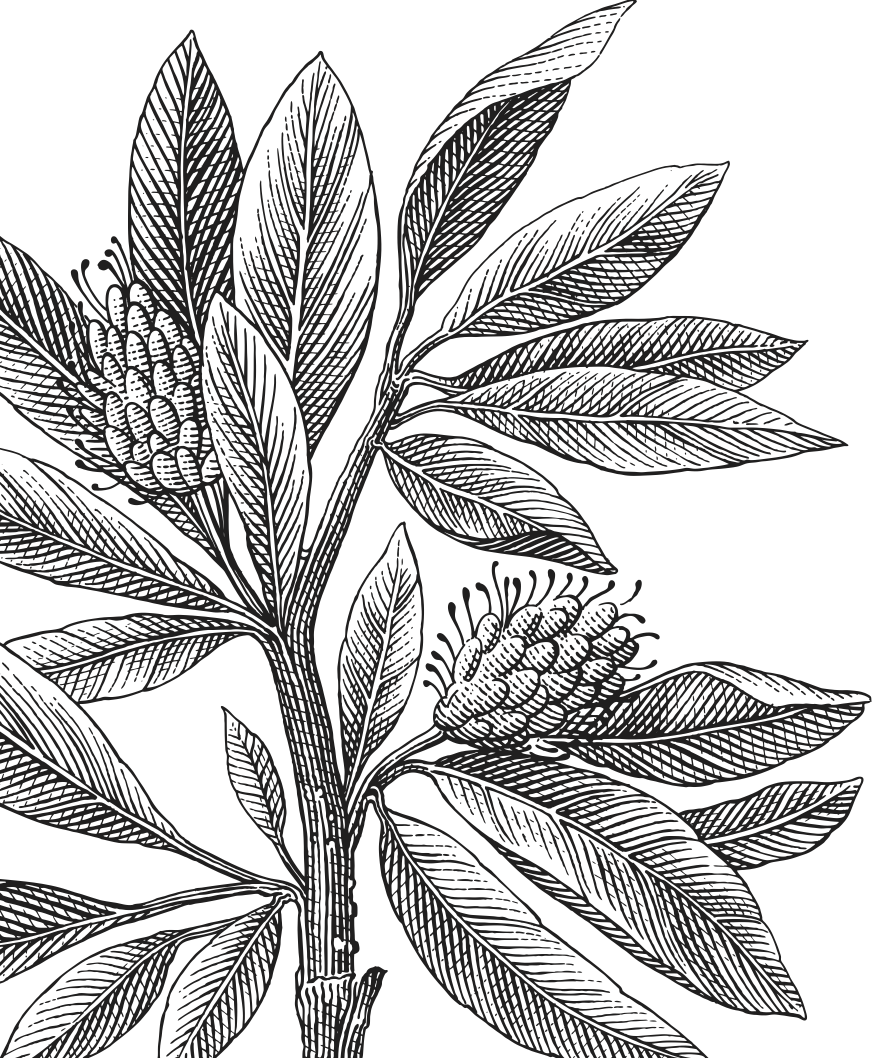
\includegraphics[keepaspectratio,scale=0.3]{img/lnu_etch.png} % Background picture
    }
}
\newcommand\BackgroundPicLogo{
    \put(30,740){
    
\includegraphics[keepaspectratio,scale=0.10]{img/logo.png} % Logo in upper left corner
    }
}

\title{	
\vspace{-8cm}
\begin{sidebar}
    \vspace{10cm}
    \normalfont \normalsize
    \Huge Bachelor Degree Project \\
    \vspace{-1.3cm}
\end{sidebar}
\vspace{3cm}
\begin{flushleft}
    \huge Title of your degree project\\ 
    \it \LARGE - Optional subtitle 
\end{flushleft}
\null
\vfill
\begin{textblock}{6}(10,13)
\begin{flushright}
\begin{minipage}{\textwidth}
\begin{flushleft} \large
\emph{Author:} Your name here\\ % Author
\emph{Supervisor:} Name of your supervisor\\ % Supervisor
%\emph{Examiner:} Dr.~Mark \textsc{Brown}\\ % Examiner (course manager)
\emph{Semester:} VT/HT 2017\\ % 
\emph{Subject:} Computer Science\\ % Subject area
\end{flushleft}
\end{minipage}
\end{flushright}
\end{textblock}
}

\date{} 

\begin{document}
\pagenumbering{gobble}
\newgeometry{left=5cm}
\AddToShipoutPicture*{\BackgroundPic}
\AddToShipoutPicture*{\BackgroundPicLogo}
\maketitle
\restoregeometry
\clearpage
%----------------------------------------------------------------------------------------
%	Abstract
%----------------------------------------------------------------------------------------
\selectlanguage{english}
\begin{abstract}
\noindent The report shall begin with a summary, called abstract. The abstract shall not be longer than a paragraph, and is not divided into more than one piece. It shall contain:

\begin {itemize}
\item A short background description to the area of your project
\item A description of the problem you investigate
\item A motivation why this problem is interesting to investigate
\item What you have done to answer the problem
\item A short summary of your results
\end {itemize}

From reading the abstract the reader should clearly understand what the report is all about. The purpose of the abstract is to make the reader interested in continue reading the report, if it covers something that the reader wants to know more about.
\newline
\newline
\textbf{Keywords: fill in some keywords for your work here. Examples: software architectures, adaptive systems, network intrusion detection, ...}
\end{abstract}

\newpage
%----------------------------------------------------------------------------------------
%	Preface
%----------------------------------------------------------------------------------------

\textbf {\large{Preface}}\\

\noindent You can have a preface in the report if you want, but it is not necessary. In this you can write more personal reflections on your degree project. In the preface you can also take the opportunity to thank the people who have been particularly helpful during the report writing, for example if you had any contact with a company that helped with the project, people that guided or helped you during the project, or your family and friends that supported you during the project. The preface shall not be longer than half a page.

%----------------------------------------------------------------------------------------
\newpage
\pagenumbering{gobble}
\tableofcontents % Table of contents
\newpage
\pagenumbering{arabic}

%----------------------------------------------------------------------------------------
%
%	Here follows the actual text contents of the report.
%
%----------------------------------------------------------------------------------------

\section{Introduction}
In this chapter you shall give an introduction to your degree project. It shall start with a broad overview of what your project is all about. Similar to the abstract, the introduction shall make the reader interested in continue reading your report. Don't be too detailed here; there are plenty of opportunities to add details in later chapters.

\subsection{Background}
After you have described your project, you shall continue with writing a background to the area your project is in. Here you describe theories necessary to understand your project and explain terms you will use in the report.

Example: if you do a project that is about evaluating software architectures, you describe what a software architecture is, why it is important to design an architecture that suits a specific software system, methods for evaluating and comparing different architectures, etc. 

\subsection{Related work}
Here you briefly describe what others have done in the field of study or how others have attempted to explain or solve the same or similar problem as you are investigating. It is okay to refer to tech articles and online blogs and portals, but you must also refer to published articles. To find articles, use the search tools listed \href{https://coursepress.lnu.se/subject/thesis-projects/tools/}{here}.

\subsection{Problem formulation}
Here you give a detailed description of the problem you intend to investigate. You can re-use the problem formulation from your project plan. You can read more about suitable problems \href{https://coursepress.lnu.se/subject/thesis-projects/problem/}{here}.

\subsection{Motivation}
Here you motivate why your problem is interesting for science, society or industry. You can re-use the motivation part from your project plan.

\subsection{Objectives}
Present a list of the objectives to do in your project. An objective shall be understandable, not too small or too large, and possible to define when it is completed or not. You have already defined objectives in your project plan. Copy and paste them here. You can read more about objectives \href{https://coursepress.lnu.se/subject/thesis-projects/objectives/}{here}.\\

\begin{tabular} {|p{1.2cm}|p{11.6cm}|} \hline
\textbf{O1} & Objective 1 ... \\ \hline
\textbf{O2} & Objective 2 ... \\ \hline
\end{tabular}\\

You are also required to make statements about tentative and expected answers to your problem. What do you think your project will result in?

Don't mention anything about method here. It will be covered in the next chapter. Note that the objectives you have defined in the project plan can change slightly during the course of the project. This is not a problem. It is often difficult to foresee everything that can occur when writing the project plan.

\subsection{Scope/Limitation}
You cannot solve everything. Here you describe what you do, and what you don't do, in your project. Limitations can for example be that you only compare some frameworks of all frameworks available on the market, that you only suggest an architecture for a specific software product and not a general architecture, or that you only include university students in a study and not a broader population sample.

\subsection{Target group}
Here you outline which target group that might be interested in your work. If you, for example, do a project about software architectures, a target group can be professional developers and architects that work with similar software systems as the system you investigated.

\subsection{Outline}
Here you outline the rest of the report. It shall contain which chapters that will follow, and what each of them is about.

\newpage

\section{Method}
\label{Method}
In your degree project you have defined a problem to investigate, and you need some problem-solving activity to answer that problem. This is what we mean with a method. We have a problem, and we need some proven and structured way of approaching and solving that problem. There is no single way that works for all problems. Researchers have learned through history that particular methods are effective for problems that share some characteristics (in terms of purpose, context or problem). You can, therefore, look at how others have answered similar problems as your own problem, and use a similar method.

There is a wide range of methods you can use in your project. The most common ones used in degree projects are:
\begin{itemize}
\item Controlled Experiment
\item Survey using questionnaires
\item Interview
\item Case Study
\item Systematic Literature Review
\item Verification and Validation 
\end{itemize}

You can read about methods \href{https://coursepress.lnu.se/subject/thesis-projects/method-overview/}{here}.

\subsection{Reliability and Validity}
Here you discuss the reliability and validity of your project. To answer your problem you use a method, collect (and possibly analyze) data, and draw conclusions from the data. 

Reliability means if others will get the same result as you if they replicate your work. Reliability problems can, for example, occur if you use the wrong method for data collection.

It is important that you only draw conclusions that are valid, i.e. that is supported by the way you have done your work and the data you have collected. 

You can read about reliability \href{https://coursepress.lnu.se/subject/thesis-projects/reliability/}{here} and about validity \href{https://coursepress.lnu.se/subject/thesis-projects/validity/}{here}. Discuss if you have any reliability issues or validity threats in your project here.

\subsection{Ethical considerations}
You are required to discuss any ethical considerations (if any) in your project. If you do an experiment you will most likely not have any ethical considerations, but in a survey ethical considerations can for example be how you make sure that the privacy of the people participating in the study is not violated (by for example removing names from the gathered data). 

\newpage

\section{Implementation}
It is common that you will develop something in your project. It can be a mobile app, a stand-alone application, a website, a game, etc. In this chapter you describe the software you have implemented. 

In some projects you don't develop anything, for example if you do a systematic literature review. In this case you remove this chapter.

\newpage

\section{Results}
In this chapter you show and describe your results. You shall only show the raw results without any analysis, and you shall not put any conclusions or opinions in the description of the results. Try to be as objective as possible. An example of results from an experiment comparing five sorting algorithms is shown in Table \ref{results} below.\\

\begin{center}
\begin{table}[ht]
\begin{center}
\begin{tabular}{ccccccc}
\hline
Run & Bubble & Quick & Selection & Insertion & Merge \\
\hline
1 & 17384 & 24 & 3258 & 3 & 30 \\
2 & 17559 & 21 & 3386 & 3 & 27 \\
3 & 17795 & 19 & 3344 & 4 & 28 \\
4 & 17484 & 20 & 3417 & 3 & 28 \\
5 & 17642 & 19 & 3358 & 3 & 30 \\
\hline
Average & 17572.8 & 20.6 & 3352.6 & 3.2 & 28.6 \\
\hline
%
\end{tabular}
\end{center}
\caption{Execution times for the five sorting algorithms on 100 000 random numbers between 0 and 10 000.}
\label{results}
\end{table}
\end{center}

What you show heavily depends on the type of method you use and what type of data you collect. Numerical data can for example be shown in both tables and graphs. A complementary graph for the sorting algorithms example is shown in Figure \ref{graph}. For a questionnaire you can show the frequency (how many participants that selected the same answer) of each possible answer to a question.

\begin{figure}[ht!]
\begin{center}
\includegraphics*[width=0.6\columnwidth]{img/graph}
\end{center}
\caption{Execution times for the five sorting algorithms shown as a graph.}
\label{graph}
\end{figure}

Note that Tables and Figures shall be labeled with chapter.number, for example Table 4.1 and Figure 1.6.

\newpage
	
\section{Analysis}
Here you give meaning to and your own opinions of the results. What conclusions can you draw from the results? It is important that you don't draw any conclusions that cannot be backed up by your data. Consider using statistical tests to back up your claims. You can read about statistical testing \href{https://coursepress.lnu.se/subject/thesis-projects/statistical-testing/}{here}. 
	
\newpage
	
\section{Discussion}
Here you discuss your findings and if your problem has been answered. Think of the project as a feedback loop. You define a problem, find a method of approaching it, conduct the study or experiment, and gather data. The data is then used to answer your problem, thus creating the loop.

You shall also discuss how your findings relate to what others have done in the field of study. Are your results similar to the findings in the related work you described in the Related work section?

This chapter is typically written in the present tense, while the previous chapters typically are written in past tense.

\newpage
		
\section{Conclusion}
In this chapter you end your report with a conclusion of your findings. What have you shown in your project? Are your results relevant for science, industry or society? How general are your results (i.e. can they be applied to other areas/problems as well)? Also discuss if anything in your project could have been done differently to possibly get better results. 

This chapter is also written in present tense.

\subsection{Future work}
You cannot do everything within the limited scope of a degree project. Here you discuss what you would do if you had continued working on your project. Are there any open questions that you discovered during the project work that you didn't have time to investigate?

\newpage


%----------------------------------------------------------------------------------------
%	References. IEEE style is used.
%
%----------------------------------------------------------------------------------------
\newpage

Here you shall include a list of all references used in your report. The reference list shall use the IEEE format. You can read about IEEE referencing \href{https://coursepress.lnu.se/subject/thesis-projects/ieee-references/}{here}. In the reference list below you can find examples of how to list a webpage \cite{courseroom}\cite{ieeeguide}, a journal article \cite{bigdata}, a book \cite{ai} and a conference proceeding (article) \cite{bigdata2}.

\hypersetup{urlcolor=black}
\bibliographystyle{IEEEtran}
\bibliography{referenser}
\newpage
%----------------------------------------------------------------------------------------
%	Appendix
%-----------------------------------------------------------------------------------------
\pagenumbering{Alph}
\setcounter{page}{1} % Reset page numbering for Appendix
\appendix

\section{Appendix 1} 
In the appendix you can put details that does not fit into the main report. Examples are source code, long tables with raw data and questionnaires.

\end{document}
